\documentclass[tikz,border=1pt]{standalone}
\usepackage{pgfplots}
\pgfplotsset{compat=1.18}
\begin{document}
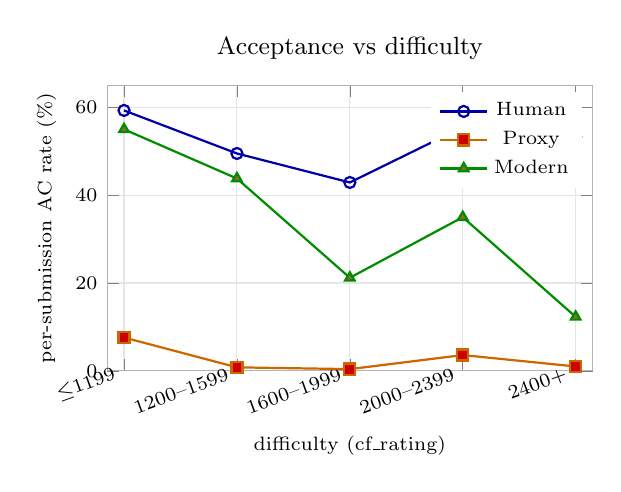
\begin{tikzpicture}
\begin{axis}[
  width=3.05in,
  height=2.05in,
  title={Acceptance vs difficulty},
  xlabel={difficulty (cf\_rating)},
  ylabel={per-submission AC rate (\%)},
  xmin=-0.15,
  xmax=4.15,
  ymin=0,
  ymax=65,
  xtick={0,1,2,3,4},
  xticklabels={{$\le$1199},{1200--1599},{1600--1999},{2000--2399},{2400+}},
  x tick label style={rotate=20,anchor=east,font=\scriptsize},
  tick label style={font=\scriptsize},
  label style={font=\scriptsize},
  title style={font=\small},
  legend style={draw=none,font=\scriptsize,at={(0.98,0.98)},anchor=north east},
  grid=major,
  grid style={draw=gray!20},
  axis line style={gray!60},
]
\addplot+[mark=o,thick,blue!65!black] coordinates {
  (0,59.3) (1,49.5) (2,42.9) (3,55.5) (4,53.3)
};
\addlegendentry{Human}
\addplot+[mark=square*,thick,orange!80!black] coordinates {
  (0,7.6) (1,0.8) (2,0.4) (3,3.6) (4,1.0)
};
\addlegendentry{Proxy}
\addplot+[mark=triangle*,thick,green!55!black] coordinates {
  (0,55.0) (1,43.8) (2,21.2) (3,35.0) (4,12.3)
};
\addlegendentry{Modern}
\end{axis}
\end{tikzpicture}
\end{document}
